\documentclass{egee}
\def\insideUG{}

%
%% Copyright (c) Members of the EGEE Collaboration. 2004-2010.
%% See http://www.eu-egee.org/partners for details on the copyright holders.
%% 
%% Licensed under the Apache License, Version 2.0 (the "License");
%% you may not use this file except in compliance with the License.
%% You may obtain a copy of the License at
%% 
%%     http://www.apache.org/licenses/LICENSE-2.0
%% 
%% Unless required by applicable law or agreed to in writing, software
%% distributed under the License is distributed on an "AS IS" BASIS,
%% WITHOUT WARRANTIES OR CONDITIONS OF ANY KIND, either express or implied.
%% See the License for the specific language governing permissions and
%% limitations under the License.
%
% external packages
\usepackage{xspace}
\usepackage{ifthen}
\usepackage{comment}

% useful definitions
\def\LB{L\&B\xspace}
\def\LBnew{\LB version 2.0\xspace}
\def\LBold{\LB version 1.x\xspace}
\def\JP{JP\xspace}
%\def\eg{e.\,g.}
\def\eg{for example\xspace}
\def\Eg{For example\xspace}
%\def\ie{i.\,e.}
\def\ie{that is\xspace}
\def\wrt{with respect to\xspace}
\def\Dash{---\penalty-1000}

\def\req{\noindent\textbf{Prerequisities:}}
\def\how{\noindent\textbf{How to run:}}
\def\what{\noindent\textbf{What to test:}}
\def\result{\noindent\textbf{Expected result:}}
\def\note{\noindent\textbf{Note:}}
\def\path#1{{\normalfont\textsf{#1}}}
\def\code#1{\texttt{#1}}
\def\ctblb#1{\code{org.glite.testsuites.ctb/LB/tests/#1}}

\specialcomment{hints}{\par\noindent\textbf{Hints: }\begingroup\slshape}{\endgroup}
%\includecomment{hints}

\long\def\TODO#1{\par\noindent\textbf{TODO:} {\sl#1}\par}
\long\def\ludek#1{}

\hyphenation{plug-in}

\newcommand{\email}[1]{\href{mailto:#1}{#1}}

\input{ver.tex}


\title{Logging and Bookkeeping}
\Subtitle{User's Guide}
\author{CESNET EGEE III JRA1 and SA3 team}
\DocIdentifier{EGEE-III....}
\Date{\today}
\Activity{JRA1: Middleware Engineering}
\DocStatus{DRAFT}
\Dissemination{PUBLIC}
\DocumentLink{http://...}

\Abstract{This user's guide explains how to use the Logging and Bookkeeping
(\LB) service from the user's point of view. The service architecture is
described thoroughly. Examples on using \LB\ event logging command to log
a~user tag and change job ACL are given, as well as \LB\ query and notification
use cases. }

\begin{document}

\begin{center}
{\bf Delivery Slip}
\end{center}
\begin{tabularx}{\textwidth}{|l|l|l|X|X|}
\hline
           & {\bf Name} & {\bf Partner} & {\bf Date} & {\bf Signature} \\
\hline
{\bf From} & Ale\v{s} K\v{r}enek & CESNET & August 1, 2008 & \\
\hline
{\bf Reviewed by} & &  & & \\

\hline
{\bf Approved by} & & & & \\
\hline
\end{tabularx}

\begin{center}
{\bf Document Change Log}
\end{center}

\begin{tabularx}{\textwidth}{|l|l|X|X|}
\hline
{\bf Issue } & {\bf Date  } & {\bf Comment } & {\bf Author  } \\   \hline
1.0.0 & August 1, 2008 & Initial version & CESNET team \\

\hline
\end{tabularx}

\begin{center}
{\bf Document Change Record}
\end{center}

\begin{tabularx}{\textwidth}{|l|l|X|}
\hline
{\bf Issue } & {\bf Item  } & {\bf Reason for Change } \\   \hline

\hline
\end{tabularx}

% Taken from:
% https://twiki.cern.ch/twiki/bin/view/EGEE/EGEEgLiteSoftwareLicense
%
\vfill{}

{\bf
Copyright} \copyright\ {\bf Members of the EGEE Collaboration. 2004.  See
\href{http://www.eu-egee.org/partners/}{http://www.eu-egee.org/partners/} for
details on the copyright holders.  

Licensed under the Apache License, Version 2.0 (the "License"); you may not use
this file except in compliance with the License.  You may obtain a copy of the
License at 

\begin{center}
\href{http://www.apache.org/licenses/LICENSE-2.0}{http://www.apache.org/licenses/LICENSE-2.0}
\end{center}

Unless required by applicable law or agreed to in writing, software distributed
under the License is distributed on an "AS IS" BASIS, WITHOUT WARRANTIES OR
CONDITIONS OF ANY KIND, either express or implied.  See the License for the
specific language governing permissions and limitations under the License.
}


\clearpage

\tableofcontents

\newpage
%
%% Copyright (c) Members of the EGEE Collaboration. 2004-2010.
%% See http://www.eu-egee.org/partners for details on the copyright holders.
%% 
%% Licensed under the Apache License, Version 2.0 (the "License");
%% you may not use this file except in compliance with the License.
%% You may obtain a copy of the License at
%% 
%%     http://www.apache.org/licenses/LICENSE-2.0
%% 
%% Unless required by applicable law or agreed to in writing, software
%% distributed under the License is distributed on an "AS IS" BASIS,
%% WITHOUT WARRANTIES OR CONDITIONS OF ANY KIND, either express or implied.
%% See the License for the specific language governing permissions and
%% limitations under the License.
%
%
%% Copyright (c) Members of the EGEE Collaboration. 2004-2010.
%% See http://www.eu-egee.org/partners for details on the copyright holders.
%% 
%% Licensed under the Apache License, Version 2.0 (the "License");
%% you may not use this file except in compliance with the License.
%% You may obtain a copy of the License at
%% 
%%     http://www.apache.org/licenses/LICENSE-2.0
%% 
%% Unless required by applicable law or agreed to in writing, software
%% distributed under the License is distributed on an "AS IS" BASIS,
%% WITHOUT WARRANTIES OR CONDITIONS OF ANY KIND, either express or implied.
%% See the License for the specific language governing permissions and
%% limitations under the License.
%
\section{\LB Architecture}

%historie: vyrobeno pro WMS v EDG, 1. a 2. verze (seq. ��sla,
%cache a dotazy na stavy), v EGEE gLite---ustabiln�n�, proxy

\LB's primary purpose is tracking WMS jobs as they are processed by
individual Grid components, not counting on the WMS to provide this data.
The information gathered from individual sources is collected, stored in
a database and made available at a single contact point. The user gets a
complete view on her job without the need to inspect several service logs
(which she may not be authorized to see in the entirety or she may not be
even aware of their existence).

While \LB keeps track of submitted and running jobs, the information is
kept by the \LB service also after the job has been finished (successfully
completed its execution, failed, or has been canceled for any reason). The 
information is usually available several days after the last event
related to the job arrived, to give user an opportunity to check the job's
final state and eventually evaluate failure reasons.

As \LB collects also information provided by the WMS, the WMS services are
no longer required to provide a job-state querying interface.  Most of the
WMS services can be even designed as stateless---they process a~job and
pass it over to another service, not keeping state information about the job
anymore.  During development and deployment of the first WMS version this
approach turned to be essential in order to scale the services to the
required extent~\cite{jgc}. 

\LB must collect information about all important events in the Grid job
life. These include transitions between components or services, results
of matching and brokerage, waiting in queue systems or start and end of
actual execution.
We decided to achieve this
goal through provision of an API (and the associated library) and
instrumenting individual WMS services and other Grid components with direct
calls to this API. But as \LB is a centralized service (there exists 
a single point where all information about a particular job must
eventually arrive), direct synchronous transfer of data could have
prohibiting impact on the WMS operation.
The temporary unavailability or overload of the remote \LB service
must not prevent (nor block) the instrumented service to perform as usual.
An asynchronous model with a clear \emph{asynchronous delivery
semantics}, see Sect.~\ref{gathering}, is used to address this issue.

As individual Grid components have only local and transient view of a
job, they are able to send only information about individual events. This
raw, fairly complex information is not 
a~suitable form to be presented to the user for frequent queries. It must
be processed at the central service and users must be presented primarily with this
processed form. This form is derived from the \emph{job state} and its
transition, not from the job events themselves. The raw information is
still available, in case more detailed insight is necessary.

While the removal of state information from (some of) the WMS services
helped to achieve the high scalability of the whole WMS, the state
information is still essential for the decisions made within the resource
broker or during the matchmaking process. 
\Eg decision on job resubmission is usually affected by the number of
previous resubmission attempts. This kind of information is currently
available in the \LB only, so the next ``natural'' requirement has been
to provide an interface for WMS (and other) services to the \LB to query
for the state information. However, this requirement contains two
contradictions: (i)~due to the asynchronous event delivery model, the \LB
information may not be up to date and remote queries may lead to unexpected
results
(or even inconsistent ones---some older information may not be available for 
one query but may arrive before a subsequent query is issued),
and (ii)~the dependence on a~remote service to provide vital state information
may block the local service if the remote one is not responding.
These problems are addressed by providing \emph{local view} on the \LB data,
see Sect.~\ref{local}.




\subsection{Concepts}


\subsubsection{Jobs and events}
To keep track of user jobs on the Grid, we first need some reliable
way to identify them. This is accomplished by assigning a unique
identifier, which we call \emph{jobid} (``Grid jobid''), to every job
before it enters the Grid. A~unique jobid is assigned, making it the
primary index to unambiguously identify any Grid job. This jobid is then
passed between Grid
components together with the job description as the job flows through
the Grid; the components themselves may have (and usually do) their
own job  identifiers, which are unique only within these components.

Every Grid component dealing with the job during its lifetime 
may be a source of information about the job. The \LB gathers information
from all the 
relevant components. This information is obtained in the form of
\LB events, pieces of data generated by Grid components, which mark
important points in the job lifetime (\eg passing of job control
between the Grid components are important milestones in job lifetime
independently on the actual Grid architecture); see Appendix~\ref{a:events}
for a~complete list. We collect those
events, store them into a database and simultaneously process them to
provide higher level view on the job's state.  The \LB collects redundant
information---the event scheme has been designed to be as redundant as
possible---and this redundancy is used to improve resiliency in a
presence of component or network failures, which are omnipresent on any
Grid. 

The \LB events themselves are structured into \emph{attribute}~=
\emph{value} pairs, the set of required and optional attributes is defined by the
event \emph{type} (or scheme). For the purpose of tracking job status on
the Grid and with the knowledge of WMS Grid middleware structure we
defined an \LB schema with specific \LB event
types (see Appendix\ref{a:events}).
The schema contains a common base, the attributes that must be assigned
to every single event. The primary key is the jobid, which is also one of
the required attributes. Among other common attributes belong currently the
timestamps of the event origin and of the event arrival to LB, 
generating component name, the event type, its priority and sequence code 
(see Sect.~\ref{evprocess}) and so on. For a complete list of attributes
see \cite{lbdg}.

While the necessary and sufficient condition for a global jobid is
to be Grid-wide unique, additional desired property relates to the
transport of events through the network: All events belonging to the same
job must be sent to the same \LB database. This must be done on a~per
message basis, as each message may be generated by a different component.
The same problem is encountered
by users when they look for information about their job---they need
to know where to find the appropriate \LB database too.
While it is possible to devise a global service where each job registers
its jobid together with the address of the appropriate database, such a
service could easily become a bottleneck. We opted for another solution,
to keep the address of the \LB database within the jobid. This way,
finding appropriate \LB database address becomes a local operation
(at most parsing the jobid) and users can use the same mechanism when
connecting to the \LB database to retrieve information about a particular
job (users know its jobid). To simplify the situation even further, 
the jobid has the form of an URL, where the protocol part is
``https'', server and port identify the machine running the appropriate 
\LB server
(database) and the path contains base64 encoded MD5 hash of random
number, timestamp, PID of the generating process and IP address of the
machine, where the jobid was generated. Jobid in this form can be
used even in the web browser to obtain information about the job,
provided the \LB database runs a web server interface. This jobid is
reasonably unique---while in theory two different job identifications can
have the same MD5 hash, the probability is low enough for this jobid to
represent a globally unique job identification.

%zaj�m� n�s job, glob�ln� id, v�echna data vzta�ena k~n�mu, syrov� ud�losti
%
%v�ce zdroj� dat pro jeden job, redundance, shrom�d�n� na jednom m�st�

\subsubsection{Event gathering}
\label{gathering}
%zdroje ud�lost�, lok�ln� semantika logov�n�, store-and-forward

As described in the previous section, information about jobs are
gathered from all the Grid components processing the job in the form
of \LB events. The gathering is based on the \emph{push} model where
the components are actively producing and sending events. The push model
offers higher performance and scalability than the pull model, where the
components are to be queried by the server. In the push model, the \LB
server does not even have to know the event sources, it is sufficient
to listen for and accept events on defined interface. 

The event delivery to the destination \LB server is asynchronous and
based on the store--and--forward model to minimize the performance
impact on component processing. Only the local processing is synchronous,
the \LB event is sent synchronously only to the nearest \LB component
responsible for event delivery. This component 
is at the worst located in the same local area network (LAN) and usually
it runs on the same host as
the producing component. The event is stored there (using persistent
storage -- disk file) and confirmation is sent back to the
producing component. From the component's point of view, the
send event operation is fast and reliable, but its success only means
the event was accepted for later delivery. The \LB delivery components
then handle the event asynchronously and ensure its delivery to the
\LB server even in the presence of network failures and host reloads.

It is important to note that this transport system does not guarantee
ordered delivery of events to the \LB server; it \emph{does} guarantee
reliable and secure delivery, however. The guarantees are statistical
only, as the protocol is not resilient to permanent disk or node crashes
nor to the complete purge of the data from local disk. Being part of the
trusted infrastructure, even the local \LB components should run on
a trusted and maintained machine, where additional reliability may be
obtained \eg by a RAID disk subsystem.

\subsubsection{Event processing}%
\label{evprocess}

%diagram stav�, mapov�n� ud�lost� na hrany

%uspo��d�n� ud�lost� -- seq. ��sla, v�etn� shallow v�tv�

% ! abstraktne, nemame jeste komponenty

% prichazeji udalosti, vice zdroju, zmenene poradi (az ztraty)
% redundantni informace
% motivace: usetrit uzivatele, hlasit agregovany stav jobu
As described in the previous section, \LB gathers raw events from various
Grid middleware components and aggregates them on a~single server
on a per-job basis.
The events contain a very low level detailed information about the job
processing at individual Grid components. This level of detail is
valuable for tracking various problems with the job and/or the
components, and as complementary events are gathered (\eg each job control
transfer is logged independently by two components), the information is
highly redundant. Moreover, the events could arrive in wrong order,
making the interpretation of raw information difficult and not
straightforward.
Users, on the other hand, are interested in a much higher view, the
overall state of their job. 

For these reasons the raw events undergo complex processing, yielding 
a~high level view, the \emph{job state}, that is the primary type of data
presented to the user.
Various job states form nodes of the job state diagram (Fig.~\ref{f:jobstat}).
See Appendix~\ref{a:jobstat} for a list of the individual states.

% stavovy automat
% obrazek: stavovy diagram

\begin{figure}[ht]
\centering
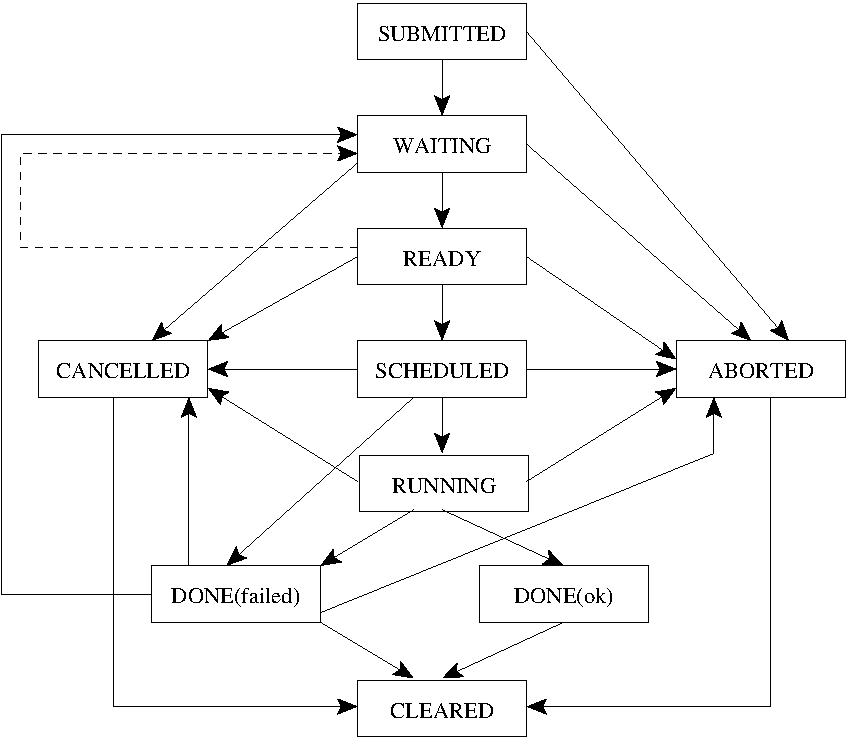
\includegraphics[width=.6\hsize]{images/wms2-jobstat}
\caption{\LB\ job state diagram}
\label{f:jobstat}
\end{figure}

% typ udalosti -> zmeny typu stavu
\LB\ defines a~\emph{job state machine} that is responsible for updating
the job state on receiving a~new event.
The logic of this algorithm is non-trivial; the rest of this section deals
with its main features.

Transitions between the job states happen on receiving events of particular
type coming from particular sources.
There may be more distinct events assigned to a~single edge of the state diagram.
For instance, the job becomes \emph{Scheduled} when it enters batch system
queue of a~Grid computing element.
The fact is witnessed by either \emph{Transfer/OK} event reported by 
the job submission service or by \emph{Accept} event reported by the computing
element. Receiving any one of these events (in any order) triggers the
state change.

% fault tolerance
This way, the state machine is highly fault-tolerant---it can cope with
delayed, reordered or even lost events.
For example, when a~job is in the \emph{Waiting} state and the \emph{Done}
event arrives, it is not treated as inconsistency but it is assumed that
the intermediate events are delayed or lost and the job state is switched
to the \emph{Done} state directly.

% udalosti nesou atributy, promitaji se do stavu 
The \LB events carry various common and event-type specific attributes,
\eg \emph{timestamp} (common) or \emph{destination} (\emph{Transfer} type).
The job state record contains, besides the major state identification,
similar attributes, \eg
an array of timestamps indicating when the job entered each state,
or \emph{location}---identification of the Grid component which is currently
handling the job.
Updating the job state attributes is also the task of the state machine,
employing the above mentioned fault tolerance---despite a~delayed event
cannot switch
the major job state back
it still may carry valuable information to update the job state attributes.

% typy jobu
Jobs monitored by \LB service may have different type. For gLite jobs, \LB supports
simple jobs and jobs representing \emph{set of jobs} -- \emph{DAGs} (with dependencies between 
subjobs described by direct acyclic graph) and \emph{collections} (without dependencies 
between subjobs). 
In these cases, subjobs are monitored in standard way, with one extensions - when job
status is changed, information is propagated also to the job representing corresponding 
collection or DAG.
Job representing collection or DAG can be used to monitor status of the set, including
information like how many subjobs is already finished etc.
Support for non-gLite jobs, namely for PBS or Condor systems, is described in section
\ref{sec:nonglite}.


\subsubsection{Event ordering}%
\label{evorder}

As described above, the ability to correctly order arriving events is
essential for the job state computation.
As long as the job state diagram was acyclic (which was true for the
initial WMS release), each event had its unique place in the expected sequence
hence event ordering could always be done implicitly from the
context.
However, this approach is not applicable once job resubmission
yielding cycles in the job state diagram was introduced.

Event ordering that would rely on timestamps assigned to events upon
their generation, assuming strict clock synchronization over the Grid,
turned to be a~naive approach.
Clocks on real machines are not precisely synchronized and there are no reliable
ways to enforce synchronization across administrative domains.

To demonstrate a problem with desynchronized clocks, that may lead to
wrong event interpretation, let us consider a~simplified example
in Tab.~\ref{t:cefail}.
%
\iffalse %stare
% usporadani udalosti -- seq. cisla
% priklad problemu
So far we assumed that the state machine is able to detect a~delayed event.
As the state diagram contains cycles, delay cannot be detected from the type
of the event only.
The simplest approach is relying on the event timestamps.
However, in the Grid environment one cannot assume strictly synchronized clocks.
Table~\ref{t:cefail} shows a~simplified example of the problem caused by delayed
clocks. 
\fi
%
\begin{table}[ht]
\begin{center}
\begin{tabular}{rlrl}
1.&WM: Accept&
6.&WM: Accept\\
2.&WM: Match $A$&
7.&WM: Match $B$\\
3.&WM: Transfer to $A$&
8.&WM: Transfer to $B$\\
4.&CE~$A$: Accept &
9.&CE~$B$: Accept \\
5.&CE~$A$: Run &
10.&CE~$B$: Run \\
\dots & $A$ dies\\
\end{tabular}
\end{center}
\caption{Simplified \LB events in the CE failure scenario}
\label{t:cefail}
\end{table}
%
We assume that the workload manager (WM) sends the job to a~computing element
(CE)~A, where it starts running but the job dies in the middle.
The failure is detected and the job is resubmitted back to the WM which sends it to CE~B then.
However, if A's clock is ahead in time and B's clock is correct (which
means behind the A's clock), the events in the right column are treated
as delayed. The state machine will interpret events incorrectly, assuming
the job has been run on B before sending it to A.
The job would always (assuming the A's events arrive before B's events to
the \LB) be reported as ``\emph{Running} at A'' despite
the real state should follow the \emph{Waiting} \dots \emph{Running} sequence.
Even the \emph{Done} event can be sent by B with a timestamp that says
this happened before the job has been submitted to A and the job state
will end with a discrepancy---it has been reported to finish on B while
still reported to run on A.

Therefore we are looking for a~more robust and general solution. We can
discover severe clock bias if the timestamp on an event is in a future
with respect to the time on an \LB server, but this is generally a dangerous
approach (the \LB server clock could be severely behind the real time).
We decided not to rely on absolute time as reported by timestamps, but to
introduce a kind of \emph{logical time} that is associated with the logic
of event generation.
The principal idea is arranging the pass through the job state 
diagram (corresponding to a~particular job life), that may include
loops, into an execution tree that represents the job history.
Closing a~loop in the pass through the state diagram corresponds
to forking a~branch in the execution tree.
The scenario in Tab.~\ref{t:cefail} is mapped to the tree in
Fig.~\ref{f:seqtree}.
The approach is quite general---any finite pass through any state
diagram (finite directed graph) can be encoded in this way.

\begin{figure}[ht]
\centering
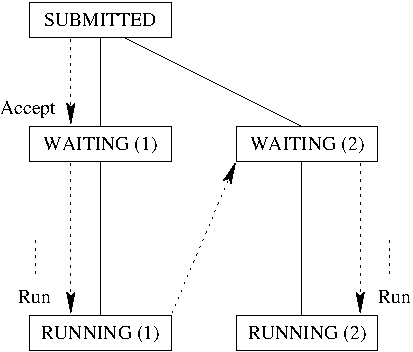
\includegraphics[scale=.833]{images/seqtree}
\caption{Job state sequence in the CE failure scenario, arranged into a~tree.
Solid lines form the tree, arrows show state transitions.}
\label{f:seqtree}
\end{figure}

Our goal is augmenting \LB events with sufficient information that
\begin{itemize}
 \item identifies uniquely a~branch on the execution tree, 
 \item determines the sequence of events on the branch, 
 \item orders the branches themselves, which means that it determines
   which one is more recent.  
\end{itemize}
If such information is available, the execution tree can be
reconstructed on the fly as the events arrive, and even delayed events
are sorted into the tree correctly.  An incoming event is considered
for job state computation only if it belongs to the most recent
branch.

The situation becomes even more complicated when 
the \emph{shallow resubmission} WM advanced feature is enabled.
In this mode WM may resubmit the job before being sure the previous attempt
is really unsuccessful, potentially creating multiple parallel instances
of the job.
The situation maps to several branches of the execution tree that
evolve really in parallel.
However, only one of the job instances becomes active (really running) finally;
the others are aborted.
Because the choice of active instance is done later, 
it may not correspond to the most recent execution branch.
Therefore, when an event indicating the choice of active instance arrives,
the job state must be recomputed, using the corresponding active branch
instead the most recent one.

Section~\ref{seqcode} describes the current implementation of event
ordering mechanism based on ideas presented here.

\subsubsection{Queries and notifications}\label{retrieve}

According to the GMA classification the user retrieves data from
the infrastructure in two modes, called
\emph{queries} and \emph{notifications} in~\LB.

Querying \LB is fairly straightforward---the user specifies query
conditions, connects to the querying infrastructure endpoint, and
receives the results. 
For ``single job'' queries, where jobid is known, the endpoint (the
appropriate \LB server) is inhered from the jobid.
More general queries must specify the \LB server explicitely,
and their semantics is intentionally restricted 
to ``all such jobs known here''.
We trade off generality for performance and reliability,
leaving the problem of finding the right query endpoint(s), the right
\LB servers, to higher level information and service-discovery services.

If the user is interested in one or more jobs, frequent polling of the
\LB server may be cumbersome for the user and creates unnecessary overload
on the sever. A notification subscription is therefore available,
allowing users to subscribe to receive notification whenever a~job 
starts matching user specified conditions.
Every subscription contains also the location of the user's
listener; 
successful subscription returns time-limited \emph{notification handle}.
During the validity period of the subscription, the \LB infrastructure
is responsible for queuing and reliable delivery of the notifications.
The user may even re-subscribe (providing the original handle) with different
listener location (\eg moving from office to home), and \LB re-routes
the notifications generated in the meantime to the new destination.
The \LB event delivery infrastructure is reused for the notification
transport.

\subsubsection{Local views}\label{local}
% motivace proxy

%As outlined in Sect.~\ref{reqs} 
WMS components are, besides logging
information into \LB, interested in querying this information back in order
to avoid the need of keeping per-job state information.
However, despite the required information is present in \LB,
the standard mode of \LB operation is not suitable for this purpose due
to the following reasons:
\begin{itemize}
\item Query interface is provided on the \LB component which gathers
events belonging to the same job but coming from different sources. 
Typically, this is a~remote service with respect to the event sources (WMS components).
Therefore the query operation is sensitive to any network failure that may
occur, blocking the operation of the querying service for indefinite time.
\item Due to the asynchronous logging semantics, there is a~non-zero time
window between successful completion of the logging call and the point in
time when the logged event starts affecting the query result.
This semantics may yield unexpected, seemingly inconsistent outcome. 
\end{itemize}

The problem can be overcome by introducing \emph{local view} on job data.
Besides forwarding events to
the server where events belonging to a~job are gathered from multiple sources,
\LB infrastructure can store the logged events temporarily
on the event source, and perform the processing described
in Sect.~\ref{evprocess}.
In this setup, the logging vs.\ query semantics can be synchronous---it is
guaranteed that a~successfully logged event is reflected in the result of
an immediately following query,
because no network operations are involved.
Only events coming from this particular physical node (but potentially
from all services running there) are considered, thus the locality of the view. 
On the other hand, certain \LB events are designed to contain redundant
information, therefore the local view on processed data (job state) 
becomes virtually complete on a~reasonably rich \LB data source like
the Resource Broker node.


\subsection{Current \LB implementation}
The principal components of the \LB service and their interactions
are shown in Figures~\ref{f:comp-gather} (gathering and transferring
\LB events) and~\ref{f:comp-query} (\LB query and notification services).

\begin{figure}[ht]
\centering
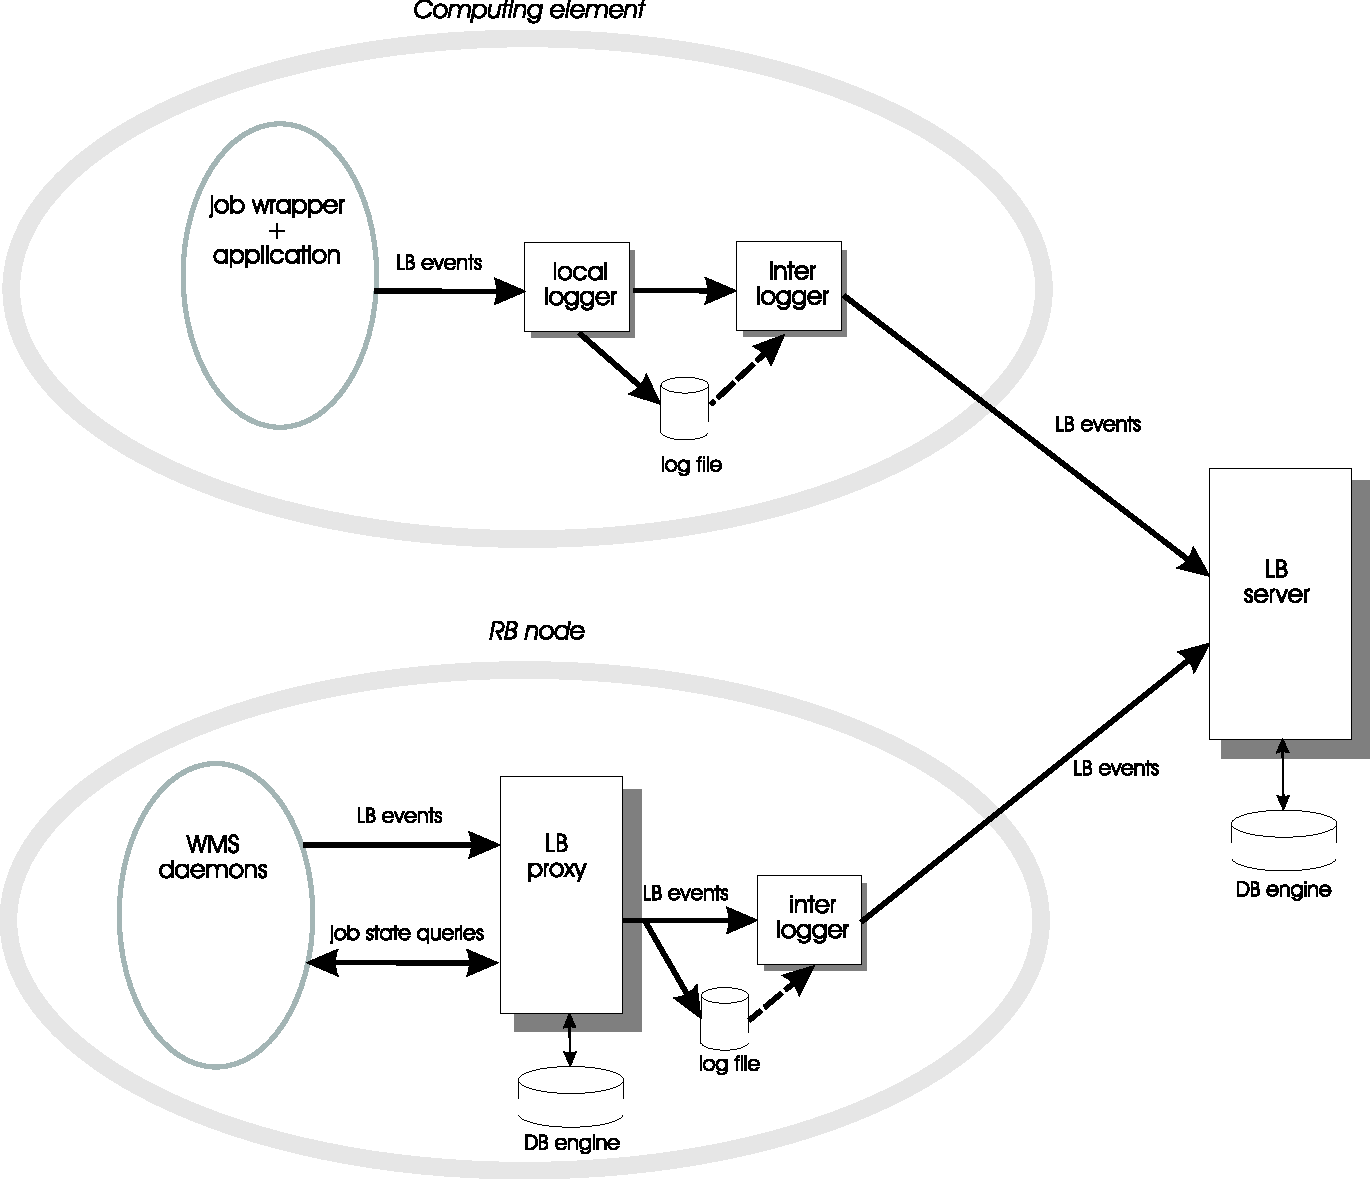
\includegraphics[scale=.5]{images/LB-components-gather}
\caption{\LB components involved in gathering and transferring the events}
\label{f:comp-gather}
\end{figure}

\input components

\subsubsection{Sequence codes for event ordering}%
\label{seqcode}

As discussed in Sect.~\ref{evorder}, sequence codes are used as logical
timestamps to ensure proper event ordering on the \LB server. The sequence code
counter is incremented whenever an event is logged and the sequence code must
be passed between individual Grid components together with the job control.
However, a single valued counter is not sufficient to support detection of
branch forks within the execution tree. When considering again the Computing
Element failure scenario described in Sect.~\ref{evorder}, there is no way to
know that the counter value of the last event logged by the failed CE A is 5
(see Table~\ref{t:cefail} on page~\pageref{t:cefail}). 

Therefore we define a~hierarchical \emph{sequence code}---an array of
counters, each corresponding to a~single Grid component class handling the job%
\footnote{Currently the following gLite components: Network Server, Workload
Manager, Job Controller, Log Monitor, Job Wrapper, and the application itself.}.
Table~\ref{t:cefail2} below shows the same scenario with a~simplified two-counter
sequence code. The counters correspond to the WM and CE component classes
and they are incremented when each of the components logs an event.
When WM receives the job back for resubmission, 
the CE counter becomes irrelevant (as the job control is on WM now),
and the WM counter is incremented again.

\begin{table}[ht]
\begin{center}
\begin{tabular}{rlrl}
1:x&WM: Accept&
4:x&WM: Accept\\
2:x&WM: Match $A$&
5:x&WM: Match $B$\\
3:x&WM: Transfer to $A$&
6:x&WM: Transfer to $B$\\
3:1&CE~$A$: Accept &
6:1&CE~$B$: Accept \\
3:2&CE~$A$: Run &
6:2&CE~$B$: Run \\
\dots & $A$ dies\\
\end{tabular}
\end{center}
\caption{The same CE failure scenario: hierarchical sequence codes.
``x'' denotes an undefined and unused value.}
\label{t:cefail2}
\end{table}

%Events on a~branch are ordered following the lexicographical order
%of the sequence codes.
%Branches are identified according to the WM counter as WM is 
%currently the only component where branching can occur.

The state machine keeps the current (highest seen) code for the job, 
being able to detect a~delayed event by simple lexicographic comparison
of the sequence codes.
Delayed events are not used for major state computation, then.
Using another two assumptions (that are true for the current
implementation):
\begin{itemize}
 \item events coming from a~single component arrive in order,
 \item the only branching point is WM,
\end{itemize}
it is safe to qualify events with lower WM counter (than the already
received one) to belong to inactive
branches, hence ignore them even for update of job state attributes.

\subsubsection{\LB data protection}
Events passed between the \LB components as well as the results of their
processing provide detailed information about the corresponding job and its
life and users obviously expect the job data provided by the \LB server to
be credible, reflecting the real jobs' operation on the Grid. Therefore, the
data must be based solely on authentic information generated by legitimate
grid components. The job data also provides information about user's
activities, which many users want to keep private. In order to provide a
sufficient level of security, the \LB infrastructure implements a security
mechanism that provides data protection and access control to the data.

All the \LB components communicate solely over secure channels whenever they
send data over a network. The TLS protocol~\cite{tls} is used for both mutual
authentication of the client and server and also encryption of the
communication. All the \LB components as well as the clients must possess a
digital certificate that they use to prove their identity. The \LB
infrastructure supports both standard X.509 certificates or proxy
certificates~\cite{proxycert} that are standard authentication mechanism in
the gLite environment. Depending on the server configuration and action
requested, the users may be required to present VOMS attributes in their
proxy certificates.

By default, access to information about a job is only allowed to the user
who submitted the job (\ie the job owner). The job owner can also assign an
access control list to his or job in the \LB specifying other users who are
allowed to read the data from \LB. The ACLs are represented in
the GridSite GACL format~\cite{gacl2} and are stored in the \LB database
along with the job information. The stored ACL are checked on each query
requesting the data. The ACLs are under control of the job owner, who can
add and remove entries in the ACL arbitrarily using the \LB API or
command-line tools (see~\ref{e:change-acl}). Each entry of an ACL can
specify either a user subject name, a name of a VOMS group, or an attribute
specified in the Full qualified attribute name format (the FQAN support is
only available in \LBnew). An ACL assigned to a job is returned as part of 
job status information.

Besides of using the ACLs, the \LB administrator can also specify a~set of
privileged users with access to all job records on a particular \LB server
(\emph{super-users}). These privileged users can \eg collect information on
usage and produce monitoring data based on the \LB information.

%Data trustworthiness - the events aren't signed, no real non-reputability or
%traceability of the event sources.


\subsection{User interaction}
\begin{figure}[ht]
\centering
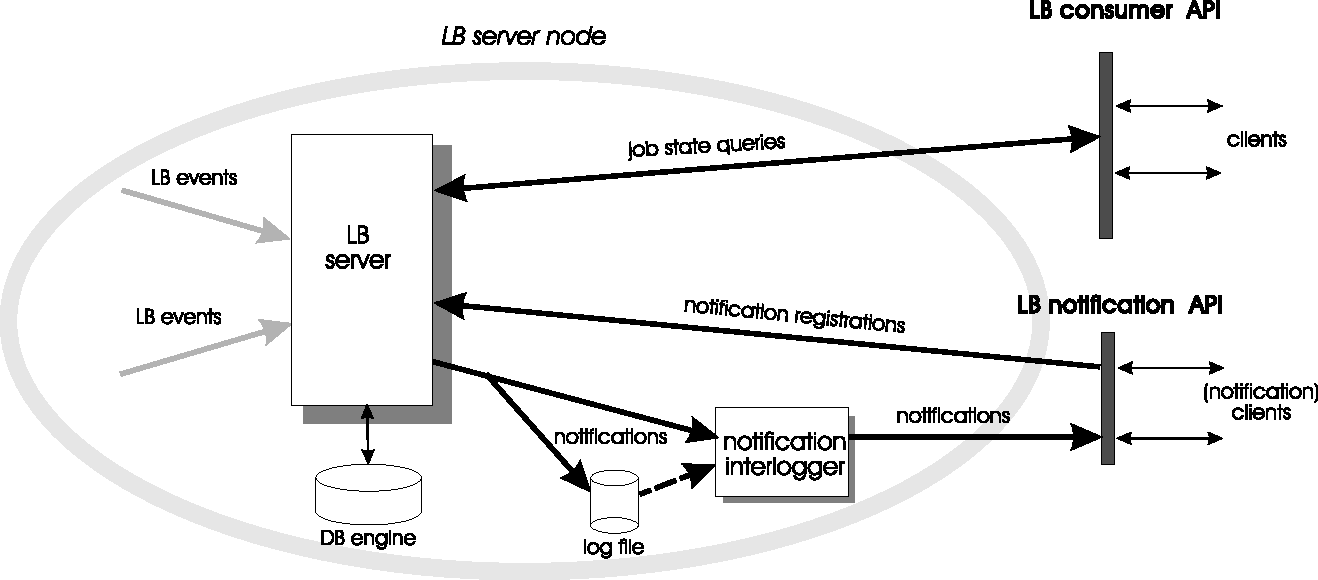
\includegraphics[scale=.5]{images/LB-components-query}
\caption{\LB queries and notifications}
\label{f:comp-query}
\end{figure}

So far we focused on the \LB internals and the interaction between its
components.
In this section we describe the interaction of users with the service.

\subsubsection{Event submission}
%implicitn� -- registrace jobu, syst�mov� ud�losti na middlewarov�ch komponent�ch
The event submission is mostly implicit,
\ie it is done transparently by the Grid middleware components
on behalf of the user.
Typically, whenever an important point in the job life is reached,
the involved middleware component logs an appropriate \LB event.
This process is not directly visible to the user.

A specific case is the initial registration of the job.
This must be done synchronously, as otherwise subsequent events logged for
the same job may be refused with a ``no such job'' error report. 
Therefore submission of a job to the WMS is the only synchronous event
logging that does not return until the job is successfully registered with
the \LB server.

% explicitn� -- user tagy, ACL
However, the user may also store information into the \LB explicitly
by logging user events---\emph{tags} (or annotations) of the
form ``name = value''.
Authorization information is also manipulated in this way. 

Description of tools for event submission and ACL manipulation 
can be found in Section \ref{s:lb-tools}.


\subsubsection{Querying information}
%\TODO{prejmenovat, aby v nazvy byly Queries}

From the user point of view, the information retrieval (\emph{query}) is the
most important interaction with the \LB service.

%dotazy na stav
The typical \LB usage are queries on the high-level job state information.
\LB supports not only single job queries, it is also possible to
retrieve information about jobs matching a specific condition.
The conditions may refer to both the \LB system attributes
and the user annotations. Rather complex query semantics can be
supported, \eg 
\emph{Which of my jobs annotated as ``apple'' or ``pear'' are already
scheduled for execution and are heading to the ``garden'' computing element?}
The \LB Developer's
Guide\cite{lbdg} provides a~series of similar examples of
complex queries.

%dotazy na ud�losti
As another option, the user may retrieve raw \LB events.
Such queries are mostly used for debugging, identification of repeating
problems, and similar purposes.
The query construction refers to event attributes rather
than job state.

The query language supports common comparison operators, and it allows
two-level nesting of conditions (logically \emph{and}-ed and \emph{or}-ed).
Our experience shows that it is sufficiently strong to cover most user
requirements while being simple enough to keep the query cost reasonable.
Complete reference of the query language can be found in~\LB Developer's Guide
\cite{lbdg}.

\subsubsection{Notifications}
The other mode of user interactions are the \LB notifications.

\LB infrastructure enables its users to be notified when something interesting happens on a \LB server
(typically job status change). It enables the user not to poll \LB server periodically to find changed
information, but confortably wait for server to inform the user.

User registers for notifications via notification client \verb'glite-lb-notify', described in Section
\ref{s:lb-notify}. 
Conditions under which the notification is sent can be specified. For example - job XY reaches status
DONE. In \LBold, one or more JOBID's are required in the condition and only a single occurence 
of a specific attribute is allowed among ANDed conditions. In \LBnew, more complex conditions are allowed.

The registration is then delivered to \LB server where it is stored.
At the same time, server generates a unique notification ID for the registration and returns it to the
user.

The registration exists only for limited amount of time. The validity is returned by \LB server together with
the notification ID when registering. During this period user can attach to server and receive notifications,
change conditions which triger notification, prolong validity of the registration, or remove the registration
from \LB server. 

While the registration is valid, user is able repeatably connect to \LB server from different places in the
network and continue receiving notifications associated with given notification ID. Notifications generated
during the time when user is connected are stored and waiting when user reconnects. 

\subsubsection{Caveats}
\LB is designed to perform well in the unreliable distributed Grid
environment.
An unwelcome but inevitable consequence of this design 
are certain contra-intuitive features in the system behavior,
namely:
\begin{itemize}
\item 
Asynchronous, possibly delayed event delivery may yield seemingly
inconsistent view on the job state \wrt\ information that is available
to the user via different channels.
\Eg the user may know that her job terminated because of monitoring the
application progress directly, but the \LB \emph{Done} events indicating
job termination are delayed so that \LB reports the job to be still
in the \emph{Running} state.

\item 
% sekven�n� ��sla -- �patn� �azen� ud�losti jsou ignorov�ny pro v�po�et stavu
Due to the reasons described in Sect.~\ref{evorder} \LB is rather sensitive
to event ordering based on sequence codes.
The situation becomes particularly complicated when there are multiple
branches of job execution.
Consequently the user may see an \LB event that is easily interpreted that
it should switch the job state, however, it has no effect in fact
because of being (correctly) sorted to an already inactive branch.

\item 
% purge -- data z~\LB\ zmiz�
\LB is not a~permanent job data storage. The data get purged from the
server on timeout, unrelated to any user's action.
Therefore, the \LB query may return ``no such job'' error message (or not
include the job in a list of retrieved jobs) even if the same previous
\LB query had no such problems.

\end{itemize}

\ludek{\subsection{Performance and scalability}
The \LB service was designed with performance and
scalability issues in mind. We have developed a series of tests of the
individual \LB components to measure the actual behavior under
stress conditions. These tests give us a good performance estimate of
the \LB service and help us identify and remove possible bottlenecks.

The testing itself is done by feeding the \LB components with events
prepared beforehand, using whatever protocol appropriate for the given
component. The feeding program uses a set of predefined events of a
typical job which we have chosen from the production \LB server
database. Timestamp is taken before the first event is sent, then the
feeding program begins sending events of individual jobs (the jobs are
all the same, the only difference is the jobid; the number of jobs used is
configurable). The tested component is instrumented in the source code
to break normal event processing at selected points (\eg discard
events immediately after being read to measure the input channel
performance, or discard events instead of sending them to the next
component, etc.). This segmentation of event processing enables to
identify places in the code which may slow down the event transfer. 
Optionally the events may be discarded by the next component in the
logical path. The last event of the last job is special termination
event, which is recognized when being discarded; then the second
timestamp is taken and the difference between the two gives us total
time necessary to pass given number of jobs through. 

Note that due to the asynchronous nature of the \LB service measuring for
example the time it takes to send given number of jobs does not give
us the required result, thus event (or job) throughput---when the
producer receives acknowledgment about successful send operation, it
is not guaranteed that the event passed through the component. 

The results shown in table~\ref{perf:results} give the overall
throughput components (events are discarded by the next component
on the path), with the exception of proxy, where the throughput to the
database is measured. It can be seen that the majority of code is fast
enough to handle even high event rates and that most components are up
to our goal to handle one million of jobs per day.  The first line
indicates how fast we are able to ``generate'' events in the feeding
program. 

\begin{table}[ht]
\begin{tabular}{l|r}
{\bf Component} & {\bf Job throughput (jobs/day)} \\
\hline
Test producer & 153,600,000 \\
Locallogger & 101,700 \\
Interlogger & 5,335,100 \\
Proxy & 1,267,110 \\
\end{tabular}
\caption{Performance testing results}
\label{perf:results}
\end{table}

During the performance testing we have identified two possible
bottlenecks:
\begin{itemize}
\item Opening connections and establishing SSL sessions is very
expensive operation. It hinders mainly the performance of locallogger,
because the current implementation uses one SSL session for
event.
\item Database operations. Storing events into database is expensive,
but inevitable; however we were able to optimize for example the
code checking for duplicated events.
\end{itemize}

In the current work we are addressing the issue of SSL operations by
introducing concept of SSL connection pools, which enables components
to reuse existing connections transparently without need to tear-down
and setup new SSL contexts. }

\subsection{Advanced use}

The usability of the \LB service is not limited to the simple tasks
described earlier. It can be easily extended to support real-time job
monitoring (not only the notifications) and the aggregate information
collected in the \LB servers is a valuable source of data used for post-mortem
statistical analysis of jobs and also the Grid infrastructure behavior.
Moreover, \LB data can be used to improve scheduling decisions.

\subsubsection{\LB and real time monitoring}
The \LB server is extended to provide quickly and without any substantial
load on the database engine the following data:
\begin{enumerate}
\item number of jobs in the system grouped by internal status
(\emph{Submitted}, \emph{Running}, \emph{Done},~\ldots),
\item number of jobs that reached final state in the last
hour,
\item associated statistics like average, maximum, and minimum time spent
by jobs in the system,
\item number of jobs that entered the WMS system in the last hour.
\end{enumerate}
\LB server can be regularly queried to provide this data to give an
overview about both jobs running on the Grid and also the behavior of the
Grid infrastructure as seen from the job (or end user) perspective.
Thus \LB\ becomes a~data source for various real-tim Grid monitoring tools.

\subsubsection{R-GMA feed}
The \LB server also supports streaming the most important data---the job
state changes---to another monitoring system. It works as the
notification service, sending information about job state changes to
a~specific listener that is the interface to a monitoring interface.
As a~particular example of such a generic service, the R-GMA feed component
has been developed. It supports sending job state changes to
the R-GMA infrastructure that is part of the Grid monitoring
infrastructure used in the EGEE Grid.

Currently, only basic information about job state changes is provided
this way, taking into account the security limitation of the R-GMA. 

\subsubsection{\LB Job Statistics}
Data collected within the \LB servers are regularly purged, complicating
thus any long term post-mortem statistical analysis. Without a Job
Provenance, the data from the \LB must be copied in a controlled way and
made available in an environment where even non-indexed queries can be
asked. 

Using the \LB Job Statistics tools, one dump file per job is created 
when the job reaches a~terminal state. These dump files can be
further processed to provide and XML encoded Job History Record%
\footnote{\url{http://egee.cesnet.cz/en/Schema/LB/JobRecord}} that
contains all the relevant information from the job life. The Job History
Records are fed into a statistical tools to reveal interesting information
about the job behavior within the Grid.

This functionality is being replaced by the direct download of all the
relevant data from the Job Provenance.

\subsubsection{Computing Element reputability rank}
\label{s:ce-rank}
Production operation of the EGEE middleware showed
that misbehaving computing elements may have significant impact on
the overall Grid performance.
The most serious problem is the ``black hole'' effect---a~CE that
accepts jobs at a~high rate but they all fail there.
Such CE usually appears to be free in Grid information services
so the resource brokers keep to assign further jobs to it.

\LB data contain sufficient information to identify similar problems.
By processing the incoming data the information
was made available as on-line auxiliary statistics like
rate of incoming jobs per CE, rate of job failure, average duration of job etc.
The implementation is lightweight, allowing very high query rate.
On the RB the statistics are available as ClassAd
functions, allowing the user to specify that similarly misbehaving
CE's should be penalized or completely avoided
when RB decides where jobs get submitted.


\subsubsection{Non-gLite event sources}
\label{sec:nonglite}

\LB has been enhanced to support also non-gLite events, namely events from PBS
or Condor batch systems \cite{hpdc07}. These events are handeled differently from gLite events,
for a complete list of the PBS and Condor events see Appendix \ref{a:events}. 
Since job states in the batch system slightly differ from the states of a job
defined in \LB (see also Appendix \ref{a:jobstat}), events are processed separately
from gLite events. Both PBS and Condor events has its own state machine that processes the
events and determines the now state of the job.

Recently, there were also attempts to use \LB system to transport different types of events: 
Certificate Revocation Lists or syslog messages. For a detailed description see 
\cite{LB4CRL}.




\newpage
\section{User tools}
\label{s:lb-tools}

In this section we give a description of the CLI tools that a regular grid user
might want to use. If not stated otherwise, the tools are distributed in the
\verb'glite-lb-client' package.

\subsection{Environment variables}

Behaviour of the commands can be changed by setting enviroment variables, specifing mostly
location of servers or setting timeouts for various operations. 
For a complete list of environment variables, their form and default value
description, see Appendix~\ref{a:environment}. Setting the environment variable
is for some commands mandatory, so reading the documentaion below and
appropriate manpages is highly recommended.


\subsection{glite-wms-job-status and glite-wms-job-logging-info}

We start with tools that are distributed in \verb'glite-wms-ui-cli-python' package
and that can be found probably on all UI machines. Description of all user
commands that are used during the job submission process (generating proxy,
creating a JDL describing the job, submitting a job, retrieving output,
cancelling a job, etc.) is beoynd this document and it can be found for example
in \cite{wmsug}. We mention here only the commands that are related to
job monitoring.

Once job has been submitted to WMS (by \verb'glite-wms-job-submit'), 
a user can retrieve the job status by
\begin{verbatim}
    glite-wms-job-status <jobId>
\end{verbatim}
or if job ID is saved in the file
\begin{verbatim}
    glite-wms-job-status -i <job_id_file>
\end{verbatim}
or if user wants to see status of all his/her jobs
\begin{verbatim}
    glite-wms-job-status --all
\end{verbatim}
List of all possible job states is summarised in Appendix \ref{a:jobstat}.

Logging details on submitted job can be accessed via
\begin{verbatim}
    glite-wms-job-logging-info -v <verbosity_level> <job_ID>
\end{verbatim}
or if job ID is saved in the file
\begin{verbatim}
   glite-wms-job-logging-info -v <verbosity_level> -i <job_id_file>
\end{verbatim}
where verbosity level can be from 0 to 3. 


\subsection{glite-lb-logevent}
\label{glite-lb-logevent}

Besides the API's \LB\ offers its users a simple command-line interface for
logging events. The command glite-lb-logevent is used for this purpose. However, it
is intended for internal WMS debugging tests in the first place and should not
be used for common event logging because of possibility of confusing \LB\
server job state automaton.

The only legal user usage is for logging \verb'UserTag' and \verb'ChangeACL' events. The following description is therefore concentrating only on options dealing with these two events.

Command usage is:

\begin{verbatim}
    glite-lb-logevent [-h] [-p] [-c seq_code] \
        -j <dg_jobid> -s Application -e <event_name> [key=value ...]
\end{verbatim}

where

\begin{tabularx}{\textwidth}{lX}
\texttt{  -h  -{}-help} &           this help message\\
\texttt{  -p  -{}-priority} &       send a priority event\\
\texttt{  -c  -{}-sequence} &       event sequence code\\
\texttt{  -j  -{}-jobid} &          JobId\\
\texttt{  -e  -{}-event} &           select event type (see -e help)\\
\end{tabularx}

\medskip

Each event specified after \verb'-e' option has different sub-options enabling to set event specific values.

Sub-options usable with \verb'UserTag' event are:


\begin{tabularx}{\textwidth}{lX}
\texttt{      -{}-name}  &          tag name\\
\texttt{      -{}-value} &          tag value\\
\end{tabularx}

\medskip

Sub-options usable with \verb'ChangeACL' event are:

\begin{tabularx}{\textwidth}{lX}
\texttt{      -{}-operation} &       operation requested to perform with ACL (add, remove)\\
\texttt{      -{}-permission} &      ACL permission to change (currently only READ)\\
\texttt{      -{}-permission\_type} & type of permission requested (0 = 'allow', 1 = 'deny')\\
\texttt{      -{}-user\_id} &         DN or VOMS parameter (in format VO:group)\\
\texttt{      -{}-user\_id\_type} &    type of information given in \verb'user_id' (DN or VOMS)\\
\end{tabularx}

\bigskip

To be able to use this command several environmental variables must be set properly. User must specify where the event should be sent. This is address and port of glite-lb-logd daemon. It is done using environmental variable \verb'EDG_WL_LOG_DESTINATION' in a form \verb'address:port'.

Because user is allowed to change ACL or add user tags only for her jobs, paths to valid X509 user credentials has to be set to authorise her. This is done using two environmental variables \verb'EDG_WL_X509_KEY' and \verb'EDG_WL_X509_CERT' in a form \verb'path_to_cred'.


%
%% Copyright (c) Members of the EGEE Collaboration. 2004-2010.
%% See http://www.eu-egee.org/partners for details on the copyright holders.
%% 
%% Licensed under the Apache License, Version 2.0 (the "License");
%% you may not use this file except in compliance with the License.
%% You may obtain a copy of the License at
%% 
%%     http://www.apache.org/licenses/LICENSE-2.0
%% 
%% Unless required by applicable law or agreed to in writing, software
%% distributed under the License is distributed on an "AS IS" BASIS,
%% WITHOUT WARRANTIES OR CONDITIONS OF ANY KIND, either express or implied.
%% See the License for the specific language governing permissions and
%% limitations under the License.
%
\subsection{glite-lb-notify}
\label{s:lb-notify}

\verb'glite-lb-notify' is a fairly simple wrapper on the \LB notification API
(see also \cite{lbdg}).
It allows to create a notification (with a restricted richness of specifying 
conditions), bind to it for receiving notifications, and drop it finally.

\LB notification is a user-initiated trigger at the server.
Whenever a job enters a state matching conditions specified with the notification,
the current state of the job is sent to the notification client.
On the other hand, the notification client is a network listener
which receives server-initiated connections to get the notifications.
Unless \verb'-s' is specified, the notification library creates the listener
socket.

Within the notification validity, clients can disappear and even migrate.
However, only a single active client for a notification is allowed.

\LB server and port to contact must be specified with GLITE\_WMS\_NOTIF\_SERVER 
environment variable.

\verb'glite-lb-notify' is supported by \LBver{2.x} and newer. In \LBver{1.x}, \verb'glite-lb-notify' 
with very limited functionality can be found in \verb'examples' directory.

\verb'glite-lb-notify' support these actions:

\begin{tabularx}{\textwidth}{lX}
\texttt{new} & Create new notification registration.\\
\texttt{bind} &  Binds an notification registration to a client.\\
\texttt{refresh} &  Enlarge notification registration validity.\\
\texttt{receive}  & Binds to an existing notification registration and listen to
server.\\
\texttt{drop}     & Drop the notification registration.\\
\end{tabularx}

For action \verb'new', command usage is:

\begin{verbatim}
  glite-lb-notify new [ { -s socket_fd | -a fake_addr } -t requested_validity
           -j jobid  { -o owner | -O }  -n network_server 
           -v virtual_organization --states state1,state2,... -c -f flags]
\end{verbatim}

For action \verb'bind', command usage is:
\begin{verbatim}
  glite-lb-notify bind [ { -s socket_fd | -a fake_addr } -t requested_validity ] 
           notifid
\end{verbatim}

For action \verb'refresh', command usage is:
\begin{verbatim}
  glite-lb-notify refresh [-t requested_validity ] notifid
\end{verbatim}

For action \verb'receive', command usage is:
\begin{verbatim}
  glite-lb-notify receive  [ { -s socket_fd | -a fake_addr } ] [-t requested_validity ] [-i timeout] [-r ] [-f field1,field2,...] [notifid]
\end{verbatim}

For action \verb'drop', command usage is:
\begin{verbatim}
   glite-lb-notify drop notifid
\end{verbatim}

where

\begin{tabularx}{\textwidth}{lX}
\texttt{  notifid} & Notification ID \\
\texttt{  -s socket\_fd} &  allows  to  pass  a opened listening socket  \\
\texttt{  -a fake\_addr} &  fake the client address \\
\texttt{  -t requested\_validity} & requested validity of the notification (in seconds)   \\
\texttt{  -j jobid} & job ID to connect notification registration with   \\
\texttt{  -o owner} & match this owner DN   \\
\texttt{  -O} & match owner on current user's DN \\
\texttt{  -n network\_server} &  match only this network server (WMS entry point)  \\
\texttt{  -v virtual\_organization} & match only jobs of this Virtual Organization  \\
\texttt{  -i timeout} & timeout to receive operation in seconds   \\
\texttt{  -f field1,field2,...} & list of status fields to print (only owner by default)   \\
\texttt{  -c} & notify only on job state change \\
\texttt{  -S, --state state1,state2,...} & match on events resulting in listed states   \\
\texttt{  -r} & refresh automatically the notification registration while receiving data\\
\end{tabularx}

For additional information see also manual page glite-lb-notify(1).

\subsubsection{Example: Registration and waiting for simple notification}
\label{e:notify}

Following steps describe basic testing procedure of the notification
system by registering a notification on any state change of this job
and waiting for notification.

Register notification for a given jobid
%(\verb'https://skurut68-2.cesnet.cz:9100/D1qbFGwvXLnd927JOcja1Q'), 
with validity 2 hours (7200 seconds):

\begin{verbatim}
  GLITE_WMS_NOTIF_SERVER=skurut68-2.cesnet.cz:9100 glite-lb-notify new \
   -j https://skurut68-2.cesnet.cz:9100/D1qbFGwvXLnd927JOcja1Q -t 7200
\end{verbatim}

returns:

\begin{verbatim}
  notification ID: https://skurut68-2.cesnet.cz:9100/NOTIF:tOsgB19Wz-M884anZufyUw 
\end{verbatim}


Wait for notification (with timeout 120 seconds):
\begin{verbatim}
  GLITE_WMS_NOTIF_SERVER=skurut68-2.cesnet.cz:9100 glite-lb-notify receive \
   -i 120 https://skurut68-2.cesnet.cz:9100/NOTIF:tOsgB19Wz-M884anZufyUw 
\end{verbatim}

returns:
\begin{verbatim}
  notification is valid until: '2008-07-29 15:04:41' (1217343881)
  https://skurut68-2.cesnet.cz:9100/D1qbFGwvXLnd927JOcja1Q        Waiting
      /DC=cz/DC=cesnet-ca/O=Masaryk University/CN=Miroslav Ruda
  https://skurut68-2.cesnet.cz:9100/D1qbFGwvXLnd927JOcja1Q        Ready
      /DC=cz/DC=cesnet-ca/O=Masaryk University/CN=Miroslav Ruda
  https://skurut68-2.cesnet.cz:9100/D1qbFGwvXLnd927JOcja1Q        Scheduled
      /DC=cz/DC=cesnet-ca/O=Masaryk University/CN=Miroslav Ruda
  https://skurut68-2.cesnet.cz:9100/D1qbFGwvXLnd927JOcja1Q        Running
      /DC=cz/DC=cesnet-ca/O=Masaryk University/CN=Miroslav Ruda
\end{verbatim}

Destroy notification:
\begin{verbatim}
  GLITE_WMS_NOTIF_SERVER=skurut68-2.cesnet.cz:9100 glite-lb-notify drop \
    https://skurut68-2.cesnet.cz:9100/NOTIF:tOsgB19Wz-M884anZufyUw
\end{verbatim}


\subsubsection{Example: Waiting for notifications on all user's jobs}

Instead of waiting for one job, user may want to accept notification about 
state changes of all his jobs.

Register notification for actual user:
\begin{verbatim}
  GLITE_WMS_NOTIF_SERVER=skurut68-2.cesnet.cz:9100 glite-lb-notify new -O
\end{verbatim}

returns:

\begin{verbatim}
  notification ID: https://skurut68-2.cesnet.cz:9100/NOTIF:tOsgB19Wz-M884anZufyUw 
\end{verbatim}

And continue with \verb'glite-lb-notify receive' similarly to previous example.
But in this case, we want to display also other information about job --
not job owner, but destination (where job is running) and location (which component is 
serving job):

\begin{verbatim}
  GLITE_WMS_NOTIF_SERVER=skurut68-2.cesnet.cz:9100 glite-lb-notify receive \
   -i 240 -f destination,location \
   https://skurut68-2.cesnet.cz:9100/NOTIF:tOsgB19Wz-M884anZufyUw
\end{verbatim}

returns:

\begin{verbatim}
  notification is valid until: '2008-07-29 15:43:41' (1217346221)

 https://skurut68-2.cesnet.cz:9100/qbRFxDFCg2qO4-9WYBiiig        Waiting
   (null) NetworkServer/erebor.ics.muni.cz/
 https://skurut68-2.cesnet.cz:9100/qbRFxDFCg2qO4-9WYBiiig        Waiting
   (null)  destination queue/erebor.ics.muni.cz/
 https://skurut68-2.cesnet.cz:9100/qbRFxDFCg2qO4-9WYBiiig        Waiting
   (null) WorkloadManager/erebor.ics.muni.cz/
 https://skurut68-2.cesnet.cz:9100/qbRFxDFCg2qO4-9WYBiiig        Waiting
   (null)  name of the called component/erebor.ics.muni.cz/
 https://skurut68-2.cesnet.cz:9100/qbRFxDFCg2qO4-9WYBiiig        Waiting
   destination CE/queue WorkloadManager/erebor.ics.muni.cz/
 https://skurut68-2.cesnet.cz:9100/qbRFxDFCg2qO4-9WYBiiig        Waiting
   destination CE/queue WorkloadManager/erebor.ics.muni.cz/
 https://skurut68-2.cesnet.cz:9100/qbRFxDFCg2qO4-9WYBiiig        Ready
   destination CE/queue destination queue/erebor.ics.muni.cz/
 https://skurut68-2.cesnet.cz:9100/qbRFxDFCg2qO4-9WYBiiig        Ready
   destination CE/queue JobController/erebor.ics.muni.cz/
 https://skurut68-2.cesnet.cz:9100/qbRFxDFCg2qO4-9WYBiiig        Ready
   destination CE/queue LRMS/destination hostname/destination instance
 https://skurut68-2.cesnet.cz:9100/qbRFxDFCg2qO4-9WYBiiig        Ready
   destination CE/queue LogMonitor/erebor.ics.muni.cz/
 https://skurut68-2.cesnet.cz:9100/qbRFxDFCg2qO4-9WYBiiig        Scheduled
   destination CE/queue LRMS/destination hostname/destination instance
 https://skurut68-2.cesnet.cz:9100/qbRFxDFCg2qO4-9WYBiiig        Running
   destination CE/queue LRMS/worknode/worker node

\end{verbatim}

\subsubsection{Example: Registering for notifications to be delivered over ActiveMQ}
\label{e:notifymsg}

Delivering notification messages over the messaging infrastructure provided by ActiveMQ is a feature introduced in \LBver{3.0}. It uses the fake address capability (\texttt{-a} option) to specify messaging topic to use when generating messages.

\begin{verbatim}
  GLITE_WMS_NOTIF_SERVER=skurut68-2.cesnet.cz:9100 glite-lb-notify new \
   -O -a x-msg://grid.emi.lbexample
\end{verbatim}

Rather than using the \LB notification API to receive messages, access the messaging infrastructure and tap into the given messaging topic (\texttt{grid.emi.lbexample} in our case).

Note that production environments can impose restrictions on topic names. In the context of EGI, for instance, prefix ``\texttt{grid.emi.}'' is mandatory. A full list of permissible topic may be obtained from the \LB Server's configuration page (Section \ref{s:findbroker}).

Also note that in case you are unsure what messaging brokers are available in your grid environment, you can read that information in the \LB Server's configuration page (Section \ref{s:findbroker}).

\subsubsection{Example: Waiting for more notifications on one socket}

The foloving example demonstrates possibility to reuse existing socket for receiving
multiple notifications. Perl script \verb'notify.pl' (available in 
examples directory) creates socket, which is then reused for all
\verb'glite-lb-notify' commands.

\begin{verbatim}
GLITE_WMS_NOTIF_SERVER=skurut68-2.cesnet.cz:9100 NOTIFY_CMD=glite-lb-notify \
 ./notify.pl -O
\end{verbatim}

returns:

\begin{verbatim}
notification ID: https://skurut68-2.cesnet.cz:9100/NOTIF:EO73rjsmexEZJXuSoSZVDg
valid: '2008-07-29 15:14:06' (1217344446)
got connection
https://skurut68-2.cesnet.cz:9100/ANceuj5fXdtaCCkfnhBIXQ        Submitted
/DC=cz/DC=cesnet-ca/O=Masaryk University/CN=Miroslav Ruda
glite-lb-notify: Connection timed out (read message)
got connection
https://skurut68-2.cesnet.cz:9100/p2jBsy5WkFItY284lW2o8A        Submitted
/DC=cz/DC=cesnet-ca/O=Masaryk University/CN=Miroslav Ruda
glite-lb-notify: Connection timed out (read message)
got connection
https://skurut68-2.cesnet.cz:9100/p2jBsy5WkFItY284lW2o8A        Waiting
/DC=cz/DC=cesnet-ca/O=Masaryk University/CN=Miroslav Ruda
\end{verbatim}


\subsubsection{Example: Waiting for notifications on jobs reaching terminal states}

This example shows how to set up notifications for jobs reaching state \emph{done} or \emph {aborted}. Since we prefer to receive just one notification per job, we will also use the \texttt{-c} option, which makes sure that notifications will be generated only on actual job state change.


\begin{verbatim}
  GLITE_WMS_NOTIF_SERVER=skurut68-2.cesnet.cz:9100 glite-lb-notify new \
   --state done,aborted -c
\end{verbatim}

returns:

\begin{verbatim}
  notification ID: https://skurut68-2.cesnet.cz:9100/NOTIF:6krjMRshTouH2n7D9t-xdg 
  valid: '2009-04-30 06:59:18 UTC' (1241074758)	
\end{verbatim}

Wait for notification (with timeout 120 seconds):
\begin{verbatim}
  GLITE_WMS_NOTIF_SERVER=skurut68-2.cesnet.cz:9100 glite-lb-notify receive \
   -i 120 https://skurut68-2.cesnet.cz:9100/NOTIF:6krjMRshTouH2n7D9t-xdg 
\end{verbatim}

returns:
\begin{verbatim}
https://skurut68-2.cesnet.cz:9100/eIbQNz3oHpv-OkYVu-cXNg	Done
    /DC=cz/DC=cesnet-ca/O=Masaryk University/CN=Miroslav Ruda
https://skurut68-2.cesnet.cz:9100/GpBy2gfIZOAXR2hKOAYGgg	Aborted
    /DC=cz/DC=cesnet-ca/O=Masaryk University/CN=Miroslav Ruda
https://skurut68-2.cesnet.cz:9100/KWXmsqvsTQKizQ4OMiXItA	Done
    /DC=cz/DC=cesnet-ca/O=Masaryk University/CN=Miroslav Ruda
https://skurut68-2.cesnet.cz:9100/O1zs50Nm1r03vx2GLyaxQw	Done
    /DC=cz/DC=cesnet-ca/O=Masaryk University/CN=Miroslav Ruda
\end{verbatim}




\subsection{HTML and plain text interface}
\label{simple}
Since the gLite jobId has the form of a unique URL, it is possible to cut and paste it directly
to the web browser to view the information about the job (esp. its status), e.g.
\begin{verbatim}
  firefox https://pelargir.ics.muni.cz:9000/1234567890
\end{verbatim}
To list all user's jobs, it is possible to query only the \LB server address, e.g.
\begin{verbatim}
  firefox https://pelargir.ics.muni.cz:9000
\end{verbatim}
To list all user's notification registration curently valid on a given \LB server, use a URL constructed as in folowing example:
\begin{verbatim}
  firefox https://pelargir.ics.muni.cz:9000/NOTIF
\end{verbatim}
A notification ID also have a form of URL. If you direct your browser to a particular notification ID, the \LB server will provide the notification details for it.
\begin{verbatim}
  firefox https://pelargir.ics.muni.cz:9000/NOTIF:1234567890
\end{verbatim}
In all cases it is necessary to have the user certificate installed in the browser.


Since \LBnew, it is also possible to obtain the above results in a machine readable 
\verb'key=value' form by adding a suffix \verb'text' to the above URLs. For example
\begin{verbatim}
  curl -3 --key $X509_USER_KEY --cert $X509_USER_CERT \
    --capath /etc/grid-security/certificates \ 
    https://pelargir.ics.muni.cz:9000?text
\end{verbatim}
or
\begin{verbatim}
  curl -3 --key $X509_USER_KEY --cert $X509_USER_CERT \
    --capath /etc/grid-security/certificates \ 
    https://pelargir.ics.muni.cz:9000/1234567890?text
\end{verbatim}

\subsection{Job state changes as an RSS feed}
The \LB includes an RSS interface allowing users to keep trace of their jobs in a very simple way using an RSS reader. The parameters of the RSS feeds are predefined, so no configuration is required.

The address of a feed is given by the URL of the \LB server and a \textit{/RSS:rss\_feed\_name} postfix, e.g.
\begin{verbatim}
   https://pelargir.ics.muni.cz:9000/RSS:finished
\end{verbatim}  

There are currently 3 feeds implemented in LB:
\begin{itemize}
 \item \textit{finished} for jobs in terminal states (Done/OK, Aborted and Canceled)
 \item \textit{running} for running jobs
 \item \textit{aborted} for aborted jobs
\end{itemize}

\subsection{Other useful tools}

For debugging purposes, low-level commands for getting \LB job status and job related events are provided in 
\verb'examples' directory (\verb'glite-lb-job_status' and \verb'glite-lb-job_log'). The same directory
contains also debugging commands for getting of all user jobs (\verb'glite-lb-user_jobs') and
CE-reputability rank (see Section \ref{s:ce-rank}, \verb'glite-lb-stats').



%\newpage
%\section{Use Cases}

This section describes usage of event-logging \LB\ command in the two
cases which are meant for the end-user: adding a~user description (tag)
to a~job, and changing a~job access control list.



User tag is an arbitrary ``name=value'' pair with which the user can 
assign additional information to a job. Further on, LB can be queried
based also on values of user tags.
% (see Sect.~\ref{tag-query}).

In order to add user tag for a job a special event \verb+UserTag+ is used. This
event can be logged by the job owner using the glite-lb-logevent command (see also
sec.\ref{cmdln_interface}). Here we suppose the command is used from user's running
 application because a correct setting of environment variables needed by 
the command is assured.

General template for adding user tag is as follows:

\begin{verbatim}
glite-lb-logevent -s Application -e UserTag    \
        -j <job_id>                         \
        -c <seq_code>                       \
        --name <tag_name>                   \
        --value <tag_value>
\end{verbatim}

where

\begin{tabularx}{\textwidth}{lX}
\verb'<job_id>'    & specifies the job to change \\
\verb'<seq_code>'   & specifies the sequence code returned by previous call
			of verb 'glite-lb-logevent'\\
\verb'<tag_name>'    & specifies the name of user tag\\
\verb'<tag_value>' & specifies the value of user tag\\
\end{tabularx}

The user application is always executed from within a JobWrapper script (part of Workload Management System \cite{WMS}). The wrapper  sets the  appropriate \verb'JobId' in the environment variable \verb'GLITE_WMS_JOBID'. The user should pass this value to the -j option of glite-lb-logevent.  Similarly, the wrapper sets an initial value of the event sequence code in the environment variable \verb'GLITE_WMS_SEQUENCE_CODE'.

If the user application calls glite-lb-logevent just once, it is sufficient to pass this value to the -c option.  However, if there are more  subsequent calls,  the  user is responsible for capturing an updated sequence code from the stdout of glite-lb-logevent and using it in subsequent calls.  The \LB\ design requires the sequence codes in  order  to  be able to sort events correctly while not relying on strictly synchronized clocks.  

The example bellow is a job consisting of 100 phases.  A user tag phase is used to log the phase  currently  being executed.  Subsequently, the user may monitor execution of the job phases as a part of the job status returned by \LB.

\begin{verbatim}
  #!/bin/sh

  for p in `seq 1 100`; do

  # log the UserTag event
  GLITE_WMS_SEQUENCE_CODE=`glite-lb-logevent -s Application
    -e UserTag
    -j $GLITE_WMS_JOBID -c $GLITE_WMS_SEQUENCE_CODE
    --name=phase --value=$p`

  # do the actual computation here
  done
\end{verbatim}


\subsubsection{Example: Changing Job Access Control List}
\label{e:change-acl}

In order to change the Access Control List (ACL) for a job, a special event
\verb'ChangeACL' is used. This event can be logged by the job owner using the
\verb'glite-lb-logevent' command (see also Sect.~\ref{glite-lb-logevent}).
The general template for changing the ACL is as follows:

\begin{verbatim}
glite-lb-logevent -e ChangeACL -s UserInterface -p -j <job_id>
        --user_id <user_id>                                             
        --user_id_type <user_id_type>                                   
        --permission READ
        --permission_type <permission_type> --operation <operation>
\end{verbatim}

where

\begin{tabularx}{\textwidth}{>{\texttt}lX}
\verb'<job_id>'    & specifies the job to change access to\\
\verb'<user_id>'   & specifies the user to grant or revoke permission. The
               parameter can be either an X.500 name
               (subject name), a VOMS group (of the form VO:Group), or a Full
               qualified attribute name (FQAN). \\
\verb'<user_id_type>' & indicates the type of the user\_id given above.
               \verb'DN', \verb'GROUP', and \verb'FQAN' can be given to
               specify X.500 name, VOMS group, or FQAN, respectively \\
\verb'<permission>' & ACL permission to change, currently only \verb'READ' is
               supported. \\
\verb'<permission_type>' & Type of permission requested. \verb'ALLOW' or
               \verb'DENY' can be specified. \\
\verb'<operation>' & Operation requested to be performed with ACL. \verb'ADD'
               or \verb'REMOVE' can be specified. \\
\end{tabularx}

Adding a user specified by his or her subject name to the ACL (\ie granting
access rights to another user):

\begin{verbatim}
glite-lb-logevent -e ChangeACL -s UserInterface -p -j <job_id>          \
        --user_id '/O=CESNET/O=Masaryk University/CN=Daniel Kouril'     \
        --user_id_type DN --permission READ --permission_type ALLOW     \
        --operation ADD
\end{verbatim}


Removing a user specified by his or her subject name from the ACL (\ie
revoking access right to another user):

\begin{verbatim}
glite-lb-logevent -e ChangeACL -s UserInterface -p -j <job_id>          \
        --user_id '/O=CESNET/O=Masaryk University/CN=Daniel Kouril'     \
        --user_id_type DN --permission READ --permission_type ALLOW     \
        --operation REMOVE
\end{verbatim}


Adding a VOMS attribute to the ACL:

\begin{verbatim}
glite-lb-logevent -e ChangeACL -s UserInterface -p -j <job_id>          \
        --user_id '/VOCE/Role=Administrator' --user_id_type FQAN        \
        --permission READ --permission_type ALLOW                       \
        --operation ADD
\end{verbatim}


Note that \LBold supported only using VOMS group names, not full FQANs,
whose support has been introduced only in \LBnew. \LBold also did not
allowed the users to use symbolic names for the values specifying ACL
setting and integers must be used instead. For example, to grant access
right on a \LBold server one has to use following syntax:

\begin{verbatim}
glite-lb-logevent -e ChangeACL -s UserInterface -p -j <job_id>          \
        --user_id '/O=CESNET/O=Masaryk University/CN=Daniel Kouril'     \
        --user_id_type 0 --permission 1 --permission_type 0 --operation 0
\end{verbatim}


\TODO{Add User Query Use Cases and Notifications Use Cases}


\appendix
\newpage
\section*{Appendix}

\section{\LB Event Types}
\label{a:events}
Complete list of all events' names together with their description follows.
% see events.tex.T
\input{events}

\newpage
\section{\LB Job States}
\label{a:jobstat}
Complete list of all job' states together with their description follows.
% see status.tex.T
\input{status}

\begin{figure}[hb]
\centering
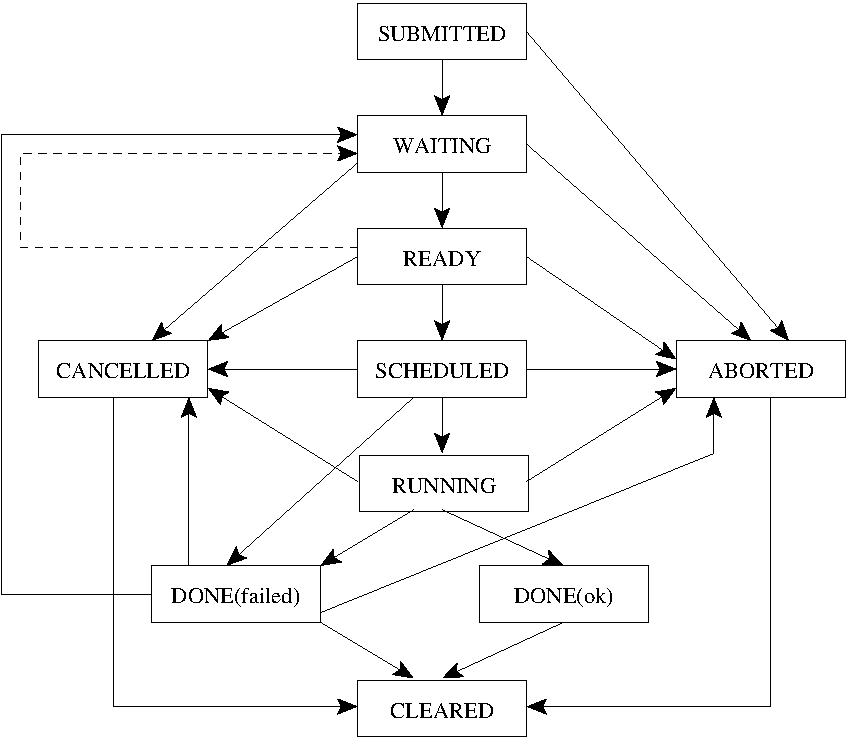
\includegraphics[width=.6\hsize]{images/wms2-jobstat}
\caption{\LB\ job state diagram}
\end{figure}

\newpage
\section{Environment variables}
\label{a:environment}
\TODO{ruda: projit}

Complete list of all environment variables affecting LB behaviour follows with 
their description and default values (if applicable).

% default values can be read especially from org.glite.lb.common/src/param.c
% and apropriate header files

\begin{tabularx}{\textwidth}{lX}
GLITE\_WMS\_LOG\_DESTINATION & 
   % see also glite/lb/log_proto.h (org.glite.lb.common/interface/log_proto.h)
   address of \verb'glite-lb-logd' daemon (for logging events), 
   in form \verb'hostname:port',
   default value is \verb'localhost:9002' \\
GLITE\_WMS\_LOG\_TIMEOUT & 
   % see also glite/lb/timeouts.h (org.glite.lb.common/interface/timeouts.h)
   timeout (in seconds) for asynchronous logging, 
   default value is \verb'120' seconds, 
   maximum value is \verb'300' seconds \\
GLITE\_WMS\_LOG\_SYNC\_TIMEOUT & 
   % see also glite/lb/timeouts.h (org.glite.lb.common/interface/timeouts.h)
   timeout (in seconds) for synchronous logging, 
   default value is \verb'120' seconds, 
   maximum value is \verb'600' seconds \\
GLITE\_WMS\_NOTIF\_SERVER & 
   address of \verb'glite-lb-bkserver' daemon (for receiving notifications)
   in form \verb'hostname:port', for receiving notifications,
   there is no default value \\
GLITE\_WMS\_NOTIF\_TIMEOUT & 
   % see also glite/lb/timeouts.h (org.glite.lb.common/interface/timeouts.h)
   timeout (in seconds) for notification registration,
   default value is \verb'120' seconds,
   maximum value is \verb'1800' seconds \\
GLITE\_WMS\_QUERY\_SERVER & 
   address of \verb'glite-lb-bkserver' daemon (for queries), 
   in form \verb'hostname:port', 
   there is no default value \\
GLITE\_WMS\_QUERY\_TIMEOUT &
   % see also glite/lb/timeouts.h (org.glite.lb.common/interface/timeouts.h)
   timeout (in seconds) for queries,
   default value is \verb'120' seconds,
   maximum value is \verb'1800' seconds \\
GLITE\_WMS\_LBPROXY\_STORE\_SOCK &
   UNIX socket location for logging to LB Proxy,
   default value is \verb'/tmp/lb_proxy_store.sock' \\
GLITE\_WMS\_LBPROXY\_SERVE\_SOCK &
   UNIX socket location for queries to LB Proxy,
   default value is \verb'/tmp/lb_proxy_serve.sock' \\
GLITE\_WMS\_LBPROXY\_USER &
   user credentials (DN) when communicating with LB Proxy,  
   there is no default value \\
X509\_USER\_CERT and X509\_USER\_KEY & 
   location of user credentials,
   default values are \verb'~/.globus/usercert.pem' and \verb'~/.globus/userkey.pem' \\
\end{tabularx}

For backward compatibility, all \verb'GLITE_WMS_*' variables can be prefixed by
\verb'EDG_WL_' instead, for example \verb'EDG_WL_LOG_DESTINATION'.


\newpage
\bibliographystyle{unsrt}
\bibliography{lbjp}

\end{document}

